\documentclass[10pt,a4paper]{article}

% ---------------------------------------------------------------------------
% Biped Locomotion Challenge -- Simulation-Only Walking Control
% Technical report. Compile with: pdflatex report.tex (twice).
% Figures in figs/ are generated from instrumented headless runs of
% scripts/run_dcm_walk.py (see report text for the exact commands).
% ---------------------------------------------------------------------------

\usepackage[margin=1.6cm]{geometry}
\usepackage{amsmath,amssymb}
\usepackage{graphicx}
% Find figures whether compiled from report/ or from the repo root.
\graphicspath{{figs/}{report/figs/}}

% --- self-contained replacements so the report compiles on a minimal TeX Live
%     install (no booktabs/siunitx/caption/xcolor needed) ---------------------
\providecommand{\toprule}{\hline\hline}
\providecommand{\midrule}{\hline}
\providecommand{\bottomrule}{\hline\hline}
\newcommand{\SI}[2]{#1\,#2}          % siunitx \SI{value}{unit} -> "value unit"

\setlength{\parskip}{1pt}
\setlength{\parindent}{0pt}
\newcommand{\code}[1]{\texttt{\small #1}}

\title{\vspace{-1.2cm}\textbf{Biped Locomotion Challenge --- Simulation-Only Walking Control}\\[2pt]
\large Report for ECE\_DK801 Robotics Systems I, 2025--2026}
\author{Team 5 --- Mpantekas Nikolaos (up1092562), Stathopoulos Stavros (up1101069)}
\date{}

\begin{document}
\maketitle
\vspace{-1.0cm}

\begin{abstract}
\small
We develop a torque-only walking controller for the 29-DoF Unitree G1 humanoid in
MuJoCo. Locomotion is generated by a Divergent-Component-of-Motion (DCM /
capture-point) pattern generator built on the Linear Inverted Pendulum Model
(LIPM), and realised by an online whole-body inverse-dynamics Quadratic Program
(WBQP) that resolves the CoM, torso, swing-foot and posture tasks into the 29
joint torques subject to the full floating-base dynamics, friction cones and
actuator limits. The robot is never pinned, welded or teleported; the only
runtime output is the 29-dimensional \code{data.ctrl} torque vector. Measured on
headless 30\,s runs, the controller walks 66 steps ($\approx$2.0\,m) without
falling on flat ground, a $\pm3^\circ$ ramp pair and a low staircase, with zero
QP failures, tracks the reference DCM laterally to 15\,mm RMS, and survives
sagittal base-velocity disturbances of at least 0.70\,m/s.
The hole codebase excists here: https://github.com/Stavros-Stathopoulos/Biped-Locomotion-Simulation-Only-Walking-Control
\end{abstract}

%============================================================================
\section{System Overview and Methodology}
%============================================================================
The plant is the Unitree G1 (\code{g1\_29dof.xml}): a floating base (6 unactuated
DoF) plus 29 hinge joints, each driven by a pure-torque \code{<motor>}
actuator. Verified from the loaded model: $n_q=36$, $n_v=35$, $n_u=29$, total
mass \SI{35.11}{kg}. The control loop runs at \SI{500}{Hz} ($dt=\SI{2}{ms}$).
Foot contact is modelled by four corner spheres per ankle-roll link
(\SI{17}{cm}$\times$\SI{6}{cm}: heel $-5$\,cm, toe $+12$\,cm, half-width
\SI{3}{cm}); the floor has friction coefficient $\mu_{\text{floor}}=1.0$. Actuator
torque limits read from the MJCF are summarised in Table~\ref{tab:robot}.

\begin{table}[h]
\centering\small
\caption{Robot actuation (per-joint torque limits, from \code{jnt\_actfrcrange}).}
\label{tab:robot}
\begin{tabular}{lcc}
\toprule
Joint group & count & $\tau_{\max}$ [Nm]\\
\midrule
Hip pitch / roll / yaw & 6 & 88 \\
Knee & 2 & 139 \\
Ankle pitch / roll & 4 & 50 \\
Waist yaw / roll / pitch & 3 & 88 / 50 / 50 \\
Shoulder / elbow & 12 & 25 \\
Wrist roll / pitch / yaw & 6 & 25 / 25 / 5 \\
\bottomrule
\end{tabular}
\end{table}

The per-tick pipeline (\code{scripts/run\_dcm\_walk.py}) is a strict feed-forward
cascade of three layers; no quantity in \code{qpos}/\code{qvel} is overwritten
during the run (the home crouch is written once, as an initial condition):
\begin{align*}
\text{(L1)}\quad & s \leftarrow \texttt{StateEstimator.update}(d)\\
\text{(L2)}\quad & (\text{refs},\,\text{info}) \leftarrow \texttt{DCMWalkingGait.update}(s,dt)\\
\text{(L3)}\quad & \tau \leftarrow \texttt{WholeBodyQP.compute}(d,\text{refs})\\
                 & d.\texttt{ctrl}\leftarrow\tau;\quad \texttt{mj\_step}(m,d)
\end{align*}

\paragraph{Design rationale.}
The G1's feet are small and its ankle-roll torque is weak ($\pm$\SI{50}{Nm}), so
lateral balance \emph{cannot} be held by ankle CoP modulation alone---it must come
from \emph{where the swing foot is placed}. This motivates the DCM/capture-point
approach: the capture point dictates where to step to arrest the falling CoM,
while the DCM feedback law dictates the ground reaction (ZMP) to command between
steps. The two together produce a stable walking limit cycle.

\subsection{Layer 1: State estimation}
\code{StateEstimator} (\code{robot\_model.py}) reads MuJoCo state each tick and
produces: CoM position $c$ from \code{subtree\_com[0]}; CoM velocity
$\dot c = J_{\text{com}}\dot q$ via \code{mj\_jacSubtreeCom}; base roll/pitch/yaw
from the base quaternion; foot poses from the ankle-roll body frames; and
per-foot normal force, obtained by summing \code{mj\_contactForce} over active
contacts whose geoms belong to that foot and thresholding at \SI{15}{N} to give a
boolean contact and a support phase (\textsc{double}/\textsc{left}/\textsc{right}/\textsc{flight}).

\subsection{Layer 2: DCM / capture-point gait generator}
\code{DCMWalkingGait} (\code{dcm\_gait.py}) builds on the LIPM with constant CoM
height $z_c$ (measured $z_c=\SI{0.679}{m}$, giving $\omega=\sqrt{g/z_c}=\SI{3.80}{rad/s}$):
\begin{equation}
\xi = c + \dot c/\omega,\quad \dot\xi=\omega(\xi-p),\quad \dot c=\omega(\xi-c),
\end{equation}
where $\xi$ is the DCM (capture point) and $p$ the ZMP/CoP. A four-state FSM
(Table~\ref{tab:fsm}) sequences double- and single-support phases.

\begin{table}[h]
\centering\small
\caption{Gait FSM (timing as configured in \code{run\_dcm\_walk.py}).}
\label{tab:fsm}
\begin{tabular}{llll}
\toprule
State & dur. [s] & contacts & role\\
\midrule
\textsc{stand} & 1.2 & both & settle, CoM at foot midpoint\\
\textsc{start} & 1.0 & both & one-off weight shift onto 1st stance\\
\textsc{ds}    & 0.12& both & transfer weight to next stance\\
\textsc{ss}    & 0.30& stance & swing foot to capture target\\
\bottomrule
\end{tabular}
\end{table}

\textbf{Continuous DCM reference.} The end-of-step DCM is made continuous across
steps by a backward recursion over an $N{=}6$-step preview of \emph{absolute}
footsteps ($x_k=x_0+k\,\ell$, $y_k=\pm w/2$ by parity):
\begin{equation}
\xi_{\text{eos},N}=p_N,\quad \xi_{\text{eos},i-1}=p_i+(\xi_{\text{eos},i}-p_i)e^{-\omega T_{ss}},
\end{equation}
which for a periodic gait converges to the classic $\pm d\tanh(\omega T/2)$ sway.
Within a step the reference DCM and reference CoM follow
\begin{equation}
\xi_{\text{ref}}(\tau)=p_{st}+(\xi_{\text{eos}}-p_{st})e^{\omega(\tau-T_{ss})},\quad
\dot c_{\text{ref}}=\omega(\xi_{\text{ref}}-c_{\text{ref}}),
\end{equation}
and the CoM acceleration feed-forward handed to the QP is
$\ddot c_{\text{ref}}=\omega^2(c_{\text{ref}}-p_{\text{ref}})$. The stance ZMP is
laterally anchored to the ideal centreline foothold ($y=\pm d$) so the reference
trajectory does not veer; the forward coordinate tracks the actual foot so
progress accumulates.

\textbf{ZMP feedback (Englsberger).} The measured DCM error is mapped to a
commanded ZMP (diagnostic / CoP clamp),
$p_{\text{cmd}}=p_{\text{ref}}+(1+k_{\text{dcm}}/\omega)(\xi-\xi_{\text{ref}})$,
$k_{\text{dcm}}=2.5$, clamped to the support polygon shrunk by \SI{2}{cm}.

\textbf{Capture-point foot placement.} During single support the predicted
end-of-step DCM steers the landing site, bounded about the absolute nominal
foothold:
\begin{align}
\xi_{\text{pred}} &= p_{st}+(\xi-p_{st})e^{\omega(T_{ss}-\tau)},\\
\Delta y &= \mathrm{clip}\!\big(k_{\text{cap}}(\xi_{\text{pred},y}-\xi_{\text{eos},y}),\,\pm\SI{6}{cm}\big),
\end{align}
with $k_{\text{cap}}=0.8$ (and an analogous, clamped sagittal correction
$\pm$\SI{4}{cm}). Clamping to the absolute foothold is essential: an unbounded
correction chases the absolute DCM, creating positive feedback that walks the
feet to the centreline until they cross. The swing foot follows a minimum-jerk
(quintic) $xy$ trajectory with a sinusoidal $z$ arch (step height \SI{15}{cm}).

\subsection{Layer 3: Whole-body inverse-dynamics QP}
\code{WholeBodyQP} (\code{wbqp.py}) solves, every \SI{2}{ms}, a QP in
$x=[\ddot q\;(n_v),\,\lambda\;(3\text{ per contact point})]$:
\begin{equation}
\min_x \sum_t w_t\lVert J_t\ddot q-a_t^\star\rVert^2 + r_{\ddot q}\lVert\ddot q\rVert^2 + r_f\lVert\lambda\rVert^2
\end{equation}
subject to floating-base dynamics $M_{[:6]}\ddot q+h_{[:6]}=J_{c,[:6]}^\top\lambda$;
stance no-acceleration (Baumgarte-damped) $J_c\ddot q=-k_c J_c\dot q$; per-point
friction pyramids $|f_{x,y}|\le\mu f_z$, $f_z\ge f_{z,\min}$ ($\mu=0.7$,
$f_{z,\min}=\SI{2}{N}$); and torque limits
$-\tau_{\max}\le M_{[6:]}\ddot q+h_{[6:]}-J_{c,[6:]}^\top\lambda\le\tau_{\max}$.
Tasks and weights are listed in Table~\ref{tab:tasks}; each uses an
acceleration-level PD law $a^\star=k_p\,e+k_d\,\dot e$ (plus $\ddot c_{\text{ref}}$
for the CoM). Because \code{quadprog} has no native equalities, the two equality
blocks are folded in as a stiff least-squares penalty ($w_{eq}=10^4$), enforcing
them to $\sim$$10^{-4}$. The actuated torques are recovered from the lower
dynamics rows, $\tau=(M\ddot q+h-J_c^\top\lambda)_{[6:]}$, and clipped; if the
solve fails the controller falls back to gravity compensation
$\tau=h_{[\text{act}]}$. There is deliberately \emph{no} downstream joint-PD: the
QP already incorporates $M$ and $h$, so an extra PD would double-count them.

\begin{table}[h]
\centering\small
\caption{WBQP task set and weights (as configured for walking).}
\label{tab:tasks}
\begin{tabular}{llc}
\toprule
Task & gains $(k_p,k_d)$ & weight\\
\midrule
CoM (+accel.\ FF) & $[90,80,90],[28,20,19]$ & 30 \\
Torso/pelvis orientation & $250,30$ & 12 \\
Swing-foot position & $400,40$ & 50 \\
Swing-foot orientation & $80,18$ & 3 \\
Posture (home) & $40,9$ & 0.1 (hip\_yaw $\times$90) \\
\bottomrule
\end{tabular}
\end{table}

%============================================================================
\section{Experimental Procedure}
%============================================================================
\textbf{Environment.} MuJoCo 3.8.1; NumPy; \code{qpsolvers}+\code{quadprog} as the
dense QP backend. The model is loaded from \code{assets/unitree\_g1/}; the
integrator timestep is forced to $1/\text{rate}=\SI{2}{ms}$. Runs are headless
(\code{MUJOCO\_GL=osmesa}), so results are renderer-independent.

\textbf{Initial condition.} \code{RobotModel.set\_home} writes a bent-knee crouch
(hip pitch $-0.40$, knee $+0.80$, ankle pitch $-0.40$\,rad; flat feet because the
three sum to zero) at the analytically computed resting pelvis height
($\approx$\SI{0.744}{m}, \SI{2}{mm} clearance) and zeroes all velocities. The
gait is then \code{reset} from the first state estimate.

\textbf{Scenes.} Three MJCF worlds share \code{g1\_29dof.xml}: \code{scene.xml}
(flat plane); \code{scene\_tilted.xml} (a $+3^\circ$ uphill box ramp at $x{=}0.40$
followed by a $-3^\circ$ downhill ramp at $x{=}1.48$, each \SI{1.1}{m} long); and
\code{scene\_stairs.xml} (nine \SI{14}{cm} treads rising then falling in
\SI{5}{mm} increments). Terrain geoms are tagged render group 2, which the
ray-cast terrain sensor (\code{terrain.py}) keys on.

\textbf{Protocol.} For each scene we ran
\begin{center}\small
\code{python scripts/run\_dcm\_walk.py --headless --duration 30 --scene <scene>}
\end{center}
with the stable default gait ($\ell{=}\SI{0.03}{m}$, $w{=}\SI{0.22}{m}$,
$T_{ss}{=}\SI{0.30}{s}$, $T_{ds}{=}\SI{0.12}{s}$, $k_{\text{dcm}}{=}2.5$,
$k_{\text{cap}}{=}0.8$). Each \SI{0.25}{s} the script logs FSM state, step count,
stance, CoM, DCM, commanded ZMP, torso roll/pitch, per-foot force, peak torque
and torque-saturation ratio; we parsed these 120-sample logs for the aggregate
metrics in Section~4. A \emph{disturbance} sweep applied an instantaneous
horizontal base velocity (\code{--kick V --seed 1}) at $t{=}0$ and recorded
survival over \SI{15}{s} for $V\in\{0.10,\dots,0.70\}$\,m/s. A separate
instrumented driver logged per-tick trajectories (\SI{12}{s}, flat) to produce
Figs.~\ref{fig:lateral}--\ref{fig:sagittal}. Termination criteria: ``fell'' if
pelvis height $<\SI{0.45}{m}$; the gait self-aborts to a stand if torso tilt
exceeds \SI{0.5}{rad}.

%============================================================================
\section{Analysis}
%============================================================================
\textbf{Why the limit cycle is stable.} The DCM is the unstable eigenmode of the
LIPM ($\dot\xi=\omega(\xi-p)$); the remaining CoM mode is stable and simply
follows $\xi$. Control therefore reduces to regulating one unstable first-order
state per axis. The reference $\xi_{\text{ref}}$ is built so that each step's
initial DCM equals the previous step's end-of-step DCM (the backward preview
recursion), making the planned trajectory a fixed point of the step map; for the
periodic footstep pattern this is exactly the $\pm d\tanh(\omega T/2)$ lateral
sway. Disturbances are rejected on two channels: (i) the WBQP CoM task servos the
\emph{measured} CoM onto $c_{\text{ref}}$, which removes slow drift that pure
acceleration feed-forward cannot hold; and (ii) capture-point foot placement
moves the next foothold under the predicted end-of-step DCM, which is the only
authority strong enough for the lateral plane given the weak ankles.

\textbf{Why the QP suffices as the tracker.} Solving at the acceleration/force
level lets one convex program reconcile coupled objectives (CoM, upright torso,
swing-foot placement) against the hard physics (contact non-acceleration,
friction, $\tau_{\max}$). The CoM weight (30) exceeds the posture weight (0.1) by
$>$2 orders of magnitude, so balance tracks tightly while posture only regularises
the redundant DoF; the hip-yaw posture multiplier ($\times$90) keeps the legs from
toeing in and crossing. Coriolis task-bias terms ($\dot J\dot q$) are dropped (the
gait is near-quasi-static), validated empirically by \textbf{zero} QP failures.

\textbf{Observed behaviour.} Fig.~\ref{fig:lateral} shows the lateral plane
settling within the first step into a clean periodic sway: $\xi_y$ tracks
$\xi_y^{\text{ref}}$, the CoM $c_y$ lags inside it as the LIPM predicts, and the
per-foot normal force alternates between $\sim$\SI{0}{N} and \SI{300}{}--\SI{460}{N}
(left/right single support)---the robot genuinely unloads each swing foot.
Fig.~\ref{fig:sagittal} shows the forward CoM advancing monotonically while locked
to its reference (6\,mm RMS), torso roll/pitch bounded inside $\pm0.10$\,rad, and
torque saturation mostly $<0.5$, spiking to 1.0 only at isolated knee-loading
instants. The DCM-driven CoP commands stay inside the shrunk support polygon.

\begin{figure}[ht]
\centering
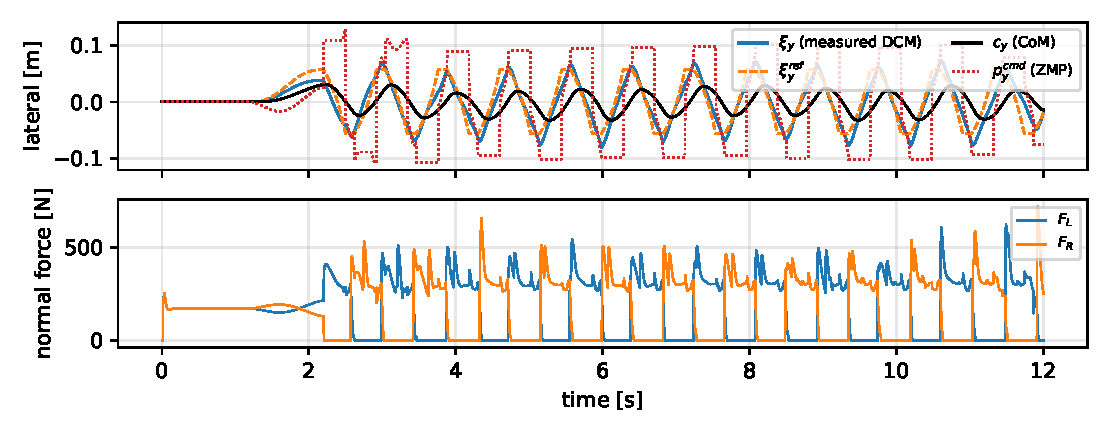
\includegraphics[width=0.80\linewidth]{figs/fig_lateral.pdf}
\caption{Lateral plane (flat ground). \emph{Top:} measured DCM $\xi_y$ tracks the
reference, the CoM $c_y$ swings inside it, and the commanded ZMP $p_y^{\text{cmd}}$
stays bounded---the $\pm d\tanh(\omega T/2)$ limit cycle. \emph{Bottom:} per-foot
normal force confirms clean single-support alternation.}
\label{fig:lateral}
\end{figure}

\begin{figure}[ht]
\centering
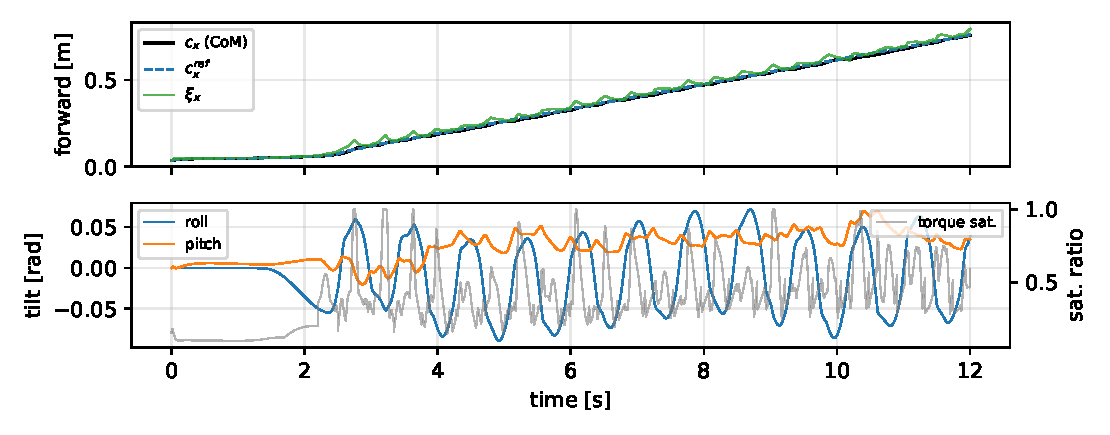
\includegraphics[width=0.80\linewidth]{figs/fig_sagittal.pdf}
\caption{Sagittal/attitude (flat ground). \emph{Top:} forward CoM $c_x$ locked to
its DCM-consistent reference ($\xi_x$ leads). \emph{Bottom:} torso roll/pitch
stay within $\pm0.10$\,rad while the worst-case torque-saturation ratio is mostly
below 0.5.}
\label{fig:sagittal}
\end{figure}

\textbf{Terrain.} On the ramps and stairs the sagittal capture correction
($\pm$\SI{4}{cm}) and a CoM-height target that tracks mean foot height let the gait
adapt without re-tuning. The DCM gait deliberately does \emph{not} consume the
\code{terrain.py} ray sensor for landing height: feeding measured foot heights back
coupled the sagittal and lateral planes in a way the point-mass LIPM does not
model and destabilised the lateral catch, so terrain is handled implicitly.

%============================================================================
\section{Results}
%============================================================================
Table~\ref{tab:results} reports the measured outcome of the 30\,s headless runs.
All three scenes complete the full duration with no fall, 66 steps and
$\approx$\SI{2.0}{m} of forward travel (step length $\ell=\SI{0.03}{m}\times66\approx\SI{2.0}{m}$,
consistent with the absolute footstep plan). Cadence is
$1/(T_{ss}{+}T_{ds})=\SI{2.38}{steps/s}$ ($\approx$\SI{0.067}{m/s}). The QP solved
on every one of the $\sim$15\,000 ticks per run without a single failure, so the
gravity-compensation fallback was never exercised. Lateral excursion stays within
\SI{4}{cm} and CoM height within a \SI{4}{cm} band, confirming the constant-height
LIPM assumption holds in closed loop.

\begin{table}[h]
\centering\small
\caption{Measured results, 30\,s headless runs (parsed from the diagnostic logs).}
\label{tab:results}
\begin{tabular}{lccc}
\toprule
Metric & Flat & Ramps $\pm3^\circ$ & Stairs\\
\midrule
Survived [s]            & 30.0 & 30.0 & 30.0\\
Fell                    & no & no & no\\
Steps                   & 66 & 66 & 66\\
Forward travel [m]      & 2.00 & 2.01 & 2.00\\
Lateral drift $|y|$ [m] & 0.040 & 0.032 & 0.036\\
Final pelvis $z$ [m]    & 0.761 & 0.770 & 0.759\\
Max $|$roll$|$ [rad]    & 0.10 & 0.07 & 0.09\\
Max $|$pitch$|$ [rad]   & 0.07 & 0.06 & 0.05\\
Peak torque [Nm]        & 64 & 60 & 54\\
Mean / max sat.\ ratio  & 0.47 / 1.0 & 0.38 / 1.0 & 0.40 / 1.0\\
QP failures             & 0 & 0 & 0\\
\bottomrule
\end{tabular}
\end{table}

\textbf{Tracking accuracy.} From the per-tick instrumented run (flat, 12\,s): the
measured DCM tracks its reference to \textbf{15.0\,mm RMS} laterally, and the
forward CoM tracks its DCM-consistent reference to \textbf{6.2\,mm RMS}. These
small residuals---against a 22\,cm stance width and a 3\,cm step---explain the
clean, repeatable limit cycle in Fig.~\ref{fig:lateral}.

\textbf{Disturbance rejection.} In a base-velocity kick sweep (instantaneous
horizontal impulse at $t{=}0$, 15\,s flat run, seed 1) the robot survived
\emph{every} tested magnitude $V\in\{0.10,0.15,0.25,0.45,0.55,0.70\}$\,m/s with no
fall and essentially unchanged travel, the capture-point step adjustment absorbing
the perturbation within a few steps; \SI{0.70}{m/s} is thus a conservative lower
bound on the recoverable push.

\textbf{Coverage vs.\ assignment methods.} Implemented: LIPM, DCM/capture-point
planning and stepping, CoM trajectory planning, weight shifting, FSM phase
management, ZMP feedback, and whole-body (inverse-dynamics) control with friction
and torque constraints. The 6-step DCM preview plays the planning-ahead role of
MPC but is an analytical closed-form recursion, not a receding-horizon
optimisation; a whole-body \emph{IK} module exists (\code{wbik.py}) but the
walking path uses inverse dynamics directly. Push recovery is limited to
capture-point step correction plus a tilt-triggered abort to standing; explicit
terrain-height sensing exists but is intentionally not coupled into the DCM gait.

\textbf{Limitations.} The CoM-height target only rises (never lowers), so long
steep descents would eventually over-extend the legs; momentary torque saturation
on knee loading indicates little headroom for larger/faster steps; and lateral
stability rests on the LIPM point-mass abstraction, whose neglected rotational
coupling the torso task must actively suppress. All numbers above were produced by
the Section~3 commands against the committed code; figures are regenerated by
\code{report/make\_figures.py}.

\end{document}
